\chapter{Zone of Proximal Development}

This is an important concept to understand because it can guide you to what you should learn next about a topic. At this given moment, we all have certain knowledge stored in our memories about specific topics. For example, I have a memory bank labeled "hepatic physiology" somewhere in my brain that contains what I know about liver physiology. This is my Present Knowledge on the topic. Since I don't know everything about liver physiology, there are still ideas/facts/concepts that I can learn and add to my memory bank. However, of all the stuff I can still learn (and there's a lot), a subset of it would be best (and easier) to learn next and other subsets would be best left alone until later. That subset that would be best (and easier) to learn next is contained in the Proximal Zone. The subsets that should be left until later are contained within the Distal Zone.

As learning proceeds, a portion of the Proximal Zone becomes part of the Present Knowledge, and as a consequence, a smaller Proximal Zone remains. Notice in the figure below how the \#1 Proximal Zone was incorporated into the present knowledge after learning occurred. Hence, over time, Present Knowledge grows but there is always a Proximal Zone present (albeit, ever changing). Also, there is always a Distal Zone present that represents knowledge to be learned later. If you knew everything there was to know about a subject, there would be no Proximal or Distal Zones (fat chance that will ever happen). Suggestions on how to involve the Zone of Proximal Development concept in your learning are listed at the very end of this page. 

\begin{figure}
	\centering
	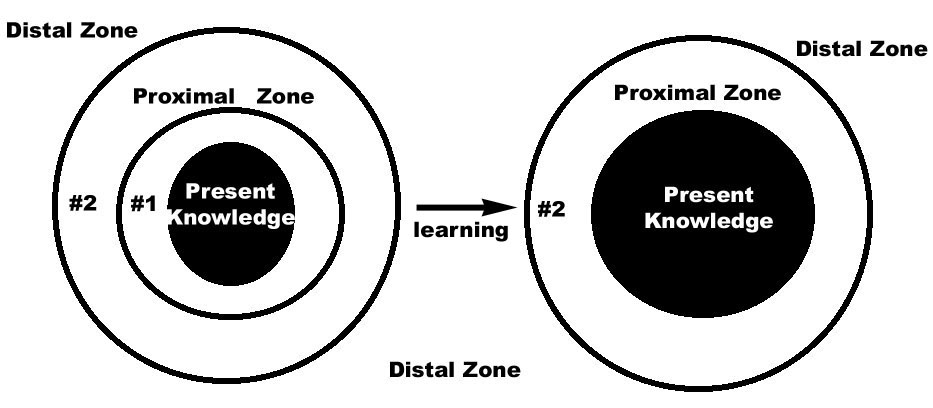
\includegraphics[width=0.80\linewidth]{./images/pz}
	\caption{Proximal Zone}
	\label{fig:pz}
\end{figure}

The take home message of this concept is that at any given time for any student (young or old), there exists material that would be the next best material to learn. For example, some courses are offered in specific sequences (i.e. Biology 101, Biology 102, etc.) and it is best to enroll in, and finish, Biology 101 before going onto Biology 102. The hard part of all of this is knowing where we stand and what we should learn next (in a given subject area). A good instructor will be able to help individual students determine if they are prepared for that instructor's course. One sad note-just because a student has completed a given course (perhaps a prerequisite) doesn't mean that the student is prepared to more forward to other subsequent courses (in a series, for example). Why? Because not every student comes out of a course learning what should have been learned (even if they passed the course). This all snowballs for some students and they find themselves in courses where they cannot learn the material because they don't have a large enough Present Knowledge structure. One last comment: The above figure also illustrates the fact that new knowledge (the material learned from the Proximal Zone) is always attached to Present Knowledge. This leads to the principle-The more you know, the easier it is to learn more (in terms of the figures, the larger the solid circle, the more area is available to attach additional knowledge). These last comments refer to Meaningful Learning and not to Rote Learning.

\section{Suggestions}

\begin{itemize}
	\item Be honest with yourself. Don't proceed to the next course in a series if you didn't learn what you should have learned in the first course. If you proceed, in this case, you will learn less from the subsequent course or courses. In the long-term, it will be like building a house on a weak foundation-sooner or later things won't work out (failure to succeed, dead-end jobs, etc.).
	\item Seek help from your instructors. See if they can determine if you are ready for their course or subsequent courses. Have them suggest corrective measures if deficiencies are noted.
	\item Make a resolution to ``learn how to learn''. It's a life-long task. 
\end{itemize}